
\documentclass[final,leqno]{siamltex704}
%\documentclass[leqno]{siamltex704}
\usepackage{epsfig}
\usepackage{amsmath,bm}
\usepackage{amssymb}
\usepackage{float}
\usepackage{tikz}
\usepackage{graphicx}
\usepackage[notcite,notref]{showkeys}
\newtheorem{algorithm}{Weak Galerkin Algorithm}
\newcommand{\bq}{{\bf q}}
\newcommand{\bn}{{\bf n}}
\newcommand{\bx}{{\bf x}}
\newcommand{\bv}{{\bf v}}
\def\bbb{{\bf b}}
\def\T{{\mathcal T}}
\def\E{{\mathcal E}}
\def\V{{\mathcal V}}
\def\W{{\mathcal W}}
\def\l{{\langle}}
\def\r{{\rangle}}
\def\jump#1{{[\![#1[\!]}}
\def\bbF{{\bf F}}
\def\bbf{{\bf f}}
\def\bn{{\bf n}}
\def\bq{{\bf q}}
\def\bV{{\bf V}}
\def\bu{{\bf u}}
\def\bv{{\bf v}}
\def\bw{{\bf w}}
\def\br{{\bf r}}
\def\bs{{\bf s}}
\def\bbQ{\mathbb{Q}}
\def\bfQ{\bf{Q}}
\def\bcurl{ \textbf{curl }}
\def\bE{{\bf E}}
\def\bB{{\bf B}}
\def\bx{{\bf x}}
\def\bU{{\bf U}}
\def\bV{{\bf V}}
\def\bJ{{\bf J}}

\def\ljump{{[\![}}
\def\rjump{{]\!]}}

\def\lavg{{\{\!\{}}
\def\ravg{{\}\!\}}}

\def\aa{\mathfrak{a}}
\def\bbQ{\mathbb{Q}}
\newcommand{\pT}{{\partial T}}
\newtheorem{defi}{Definition}[section]
\def\3bar{{|\hspace{-.02in}|\hspace{-.02in}|}}
%\setlength{\textwidth}{6truein} \setlength{\textheight}{8truein}
%\voffset=-0.55truein
%\hoffset=-0.65truein
\renewcommand{\ldots}{\dotsc}
\setlength{\parskip}{1\parskip}

\usepackage{titlesec}
\setcounter{secnumdepth}{4}
\titleformat{\paragraph}
{\normalfont\normalsize\bfseries}{\theparagraph}{1em}{}
\titlespacing*{\paragraph}
{0pt}{3.25ex plus 1ex minus .2ex}{1.5ex plus .2ex}


\title{Discontinuous Galerkin Sparse Grids Methods for Run-Away Electron Model}


\author{
}

\begin{document}

\maketitle

\begin{abstract}

\end{abstract}

\begin{keywords}

\end{keywords}

\begin{AMS}
Primary: 65N15, 65N30; Secondary: 35J50
\end{AMS}
\pagestyle{myheadings}

% Pitch Angle Dynamics
\section{Pitch Angle Dynamics}
\subsection{Electric Field Acceleration}
The governing equation is described as follows:
\begin{eqnarray}
\frac{\partial f}{\partial t} = -\frac{\partial}{\partial \xi}[(1-\xi^2)f],
\end{eqnarray}
with
\begin{eqnarray}
f(\xi,t=0)=f_0(\xi),\ f(\xi=\pm 1,t)=0.
\end{eqnarray}

\subsubsection{Numerical Scheme}
In this section, we shall consider the following hyperbolic equations.
Let the domain $\Omega\times(0,T)$ with $\Omega=[-1,1]$, the following problem will be considered in this paper,
\begin{eqnarray}
&&\frac{\partial f}{\partial t} = -\frac{\partial}{\partial x}(1-x^2)f,\mbox{ in }\Omega\label{eq:hyper-pde}%\\
%&&(1-x^2)\frac{\partial f}{\partial x}|_{x=\pm 1} = 0.\label{eq:hyper-bc}
\end{eqnarray}
The DG method will be applied to approximate the above equation. The scheme will be described as follows:
\begin{eqnarray*}
\sum_j\bigg(\int_{I_j}\big(\frac{\partial f_h}{\partial t} w-(1-x^2)f_h\frac{\partial w}{\partial x}\big) dx + (\tilde{F}_{j+1/2})(w)_{j+1/2}^- -(\tilde{F}_{j-1/2})(w)_{j-1/2}^+ \bigg)= 0.
\end{eqnarray*}
The upwind flux has been chosen as
$\tilde{F}_{j+1/2}=(1-x_{j+1/2})f_{j+1/2}^-$ and $\tilde{F}_{j-1/2}=(1-x_{j-1/2})f_{j-1/2}^-$.

Thus, the matrix form reads
\begin{eqnarray*}
\dfrac{{\bf dF}_h}{dt} =& \mathbb{B}{\bf F}_h.
\end{eqnarray*}

%---------------------------
% Numerical Example
%---------------------------
\subsubsection{Numerical Test}
The general analytical solution of this problem is
\begin{eqnarray*}
f(x,t)&=&\frac{1-\phi^2}{1-x^2}f_0(\phi),\
\phi(x,t)=\tanh(\tanh^{-1}x-t).
\end{eqnarray*}

\paragraph{Test 1}\label{Num-2}
In this test, we shall use $f_0=1$ as initial condition.

\begin{figure}[H]
\centering
\begin{tabular}{c}
  \includegraphics[width=.95\textwidth]{./hyper-cf-Test1_v2}
  \end{tabular}
\caption{Test \ref{Num-2}: Plot for solutions for Lev = 5, Deg = 5 of Central flux at time = 0.5, 1, 2, 3.}
\end{figure}


%\begin{figure}[H]
%\centering
%\begin{tabular}{c}
%  \includegraphics[width=.95\textwidth]{./hyper-cf-Test1}
%  \end{tabular}
%\caption{Test \ref{Num-2}: Plot for solutions for Lev = 5, Deg = 5 of Central flux at time = 0.5, 1, 2, 3.}
%\end{figure}

\begin{figure}[H]
\centering
\begin{tabular}{c}
  \includegraphics[width=.95\textwidth,height=.65\textwidth]{./hyper-uf-Test1_v2}
  \end{tabular}
\caption{Test \ref{Num-2}: Plot for solutions for Lev = 5, Deg = 5 of upwind flux at time = 0.5, 1, 2, 3.}
\end{figure}

%\begin{figure}[H]
%\centering
%\begin{tabular}{c}
%  \includegraphics[width=.95\textwidth]{./hyper-uf-Test1}
%  \end{tabular}
%\caption{Test \ref{Num-2}: Plot for solutions for Lev = 5, Deg = 5 of upwind flux at time = 0.5, 1, 2, 3.}
%\end{figure}


\paragraph{Test 2}\label{Num-3}
In this test, we shall use $f_0=\exp(-x^2/\sigma^2),\ \sigma=0.1$ as initial condition. 
%k=2 T=0.5
%2 2.7454e-01   6.2949e-01

%\begin{verbatim}
%CF
%2 3.5893e-01   9.2580e-01
%3 1.5262e-01   4.4423e-01
%4 1.2866e-02   2.5458e-02
%5 2.8658e-04   8.9971e-04
%UF
%k=3, T=0.5
%2 1.8697e-01   5.2381e-01
%3 5.0580e-02   1.2419e-01
%4 6.5368e-03   1.6838e-02
%5 4.4662e-04   1.7248e-03
%\end{verbatim}

%\begin{figure}[H]
%\centering
%\begin{tabular}{c}
%  \includegraphics[width=.95\textwidth]{./hyperbolic-k2-compare}
%  \end{tabular}
%\caption{Test \ref{Num-3}: Plot for solutions for Lev = 4, T = 0.5.}
%\end{figure}
%
%\begin{figure}[H]
%\centering
%\begin{tabular}{c}
%  \includegraphics[width=.95\textwidth]{./hyperbolic-k4}\\
%  \includegraphics[width=.95\textwidth]{./hyperbolic-k4-zoom}
%  \end{tabular}
%\caption{Test \ref{Num-3}: Plot for solutions for Deg = 4, T = 0.5 for upwind flux.}
%\end{figure}
%
%\begin{figure}[H]
%\centering
%\begin{tabular}{c}
%  \includegraphics[width=.95\textwidth]{./hyperbolic-k4-CF}\\
%  \includegraphics[width=.95\textwidth]{./hyperbolic-k4-CF-Zoom}
%  \end{tabular}
%\caption{Test \ref{Num-3}: Plot for solutions for Deg = 4, T = 0.5 for central flux.}
%\end{figure}

\begin{figure}
\centering
\begin{tabular}{c}
  \includegraphics[width=.95\textwidth,height=0.65\textwidth]{./hyper-CF-Test2_v2}
  \end{tabular}
\caption{Test \ref{Num-3}: Plot for solutions for Lev = 5, Deg = 5 of Central flux at time = 0.5, 1, 2, 3.}
\end{figure}


%\begin{figure}[H]
%\centering
%\begin{tabular}{c}
%  \includegraphics[width=.95\textwidth]{./hyper-cf-Test2}
%  \end{tabular}
%\caption{Test \ref{Num-3}: Plot for solutions for Lev = 5, Deg = 5 of Central flux at time = 0.5, 1, 2, 3.}
%\end{figure}

\begin{figure}
\centering
\begin{tabular}{c}
  \includegraphics[width=.95\textwidth]{./hyper-UF-Test2_v2}
  \end{tabular}
\caption{Test \ref{Num-3}: Plot for solutions for Lev = 5, Deg = 5 of upwind flux at time = 0.5, 1, 2, 3.}
\end{figure}

\paragraph{Test 3}\label{Num-4}
Next, we test the adaptive method for this test. The initial condition is chosen as Test \ref{Num-3}. In this test, we have use the Hash table and leaf hash table. Hash table contains all the grids $\Omega^{n}_\ell$, and the leaf hash only consist of the grids without children. 

The adaptive algorithm is as follows: for chosen value of $\epsilon>0$ and $\eta>0$
\begin{itemize}
\item[Step 1.] We start with previous (initial) mesh and solution ${\bf F}^{n}$
\item[Step 2.] Pre-predict the solution by Euler time stepping method
$${\bf F}^{(p)} = {\bf F}^{n}+\Delta t \mathbb{B}{\bf F}^{n}$$
\item[Step 3.] Refinement: if the coefficient $|{\bf F}^{(p)}_j|>\epsilon$, we add additional resolution to the grid. The checking up procedure is for the global grids. But we only add the non-exist grid. Then the global grid and leaf grid will be modified accordingly.
\item[Step 4.] Use 3-rd Runge-Kutta method to compute ${\bf F}^{n+1}$
\item[Step 5.] Coarsening: if the coefficient of $|{\bf F}^{n+1}_j|>\eta$, we coarsen the grid. The checking up procedure is only carried out for the leaf grids. Then the global grid and leaf grid will be modified accordingly.
\item[Step 6.] Go to Step 2 until end of time stepping
\end{itemize}

\begin{figure}[H]
\centering
\begin{tabular}{c}
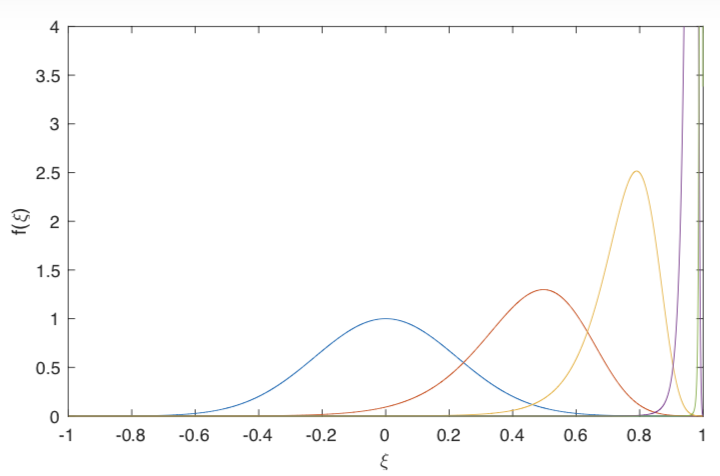
\includegraphics[width=.95\textwidth,height=.3\textwidth]{./Fig_notes/Fig2_note}\\
  \includegraphics[width=.95\textwidth,height=.6\textwidth]{./HyperAdap_Lev4_Deg2}
  \end{tabular}
\caption{Test \ref{Num-3}: Plot for solutions for Lev = 4, Deg = 2 for adaptive method.}
\end{figure}


%\begin{figure}[H]
%\centering
%\begin{tabular}{c}
%  \includegraphics[width=.95\textwidth]{./hyper-uf-Test2}
%  \end{tabular}
%\caption{Test \ref{Num-3}: Plot for solutions for Lev = 5, Deg = 5 of upwind flux at time = 0.5, 1, 2, 3.}
%\end{figure}

\subsection{Collision}

The evolution of the pitch angle dependence of $f$ in the presence of only collisions is governed by the equation:
\begin{eqnarray}
\frac{\partial f}{\partial t} = \frac{\partial}{\partial\xi}[(1-\xi^2)\frac{\partial f}{\partial\xi}]
\end{eqnarray}


% LDG
\subsubsection{Numerical Scheme of Local Discontinuous Galerkin Methods}
Let the domain $\Omega\times(0,T)$ with $\Omega=[-1,1]$, the following problem will be considered in this paper,
\begin{eqnarray}
&&\frac{\partial f}{\partial t} = \frac{\partial}{\partial x}(1-x^2)\frac{\partial f}{\partial x},\mbox{ in }\Omega\label{eq:pde}\\
&&(1-x^2)\frac{\partial f}{\partial x}|_{x=\pm 1} = 0.\label{eq:bc}
\end{eqnarray}


We rewrite Eq. (\ref{eq:pde}) as the following system
\begin{eqnarray}
f_t-q_x=0,\ q-(1-x^2)f_x=0.
\end{eqnarray}
First, we divide $[-1,1]$ into $N$ cells
\begin{eqnarray*}
-1=x_{1/2}\le x_{3/2}\le \cdots\le x_{N+1/2}=1,
\end{eqnarray*}
and denote
$$
I_j=(x_{j-1/2},x_{j+1/2}),\ x_j=(x_{j-1/2},x_{j+1/2})/2,\ h_j=x_{j+1/2}-x_{j-1/2}
$$
as the cells, cell centers and cell lengths.

Define the discontinuous Galerkin finite element space as
\begin{eqnarray}
V_h^k=\{v:v|_{I_j}\in P^k(I_j), j=1,\cdots,N\},
\end{eqnarray}
where $P^k(I_j)$ denotes the space of polynomials in $I_j$ of degree at most $k$.

The numerical scheme is to find $f_h,q_h\in V_h^k$ such that, for all test functions $w,p\in V_h^k$, we have
\begin{eqnarray}
&&\int_{I_j}\frac{\partial f_h}{\partial t}wdx+\int_{I_j}q_h\frac{\partial w}{\partial x}dx-\hat{Q}_{j+1/2}(w)^-_{j+1/2}+\hat{Q}_{j-1/2}(w)^+_{j-1/2}=0,\label{eq:ldg-1}\\
&&\int_{I_j}q_h p-2xf_h p+(1-x^2)f_h\frac{\partial p}{\partial x}dx-\hat{F}_{j+1/2}(p)^-_{j+1/2}+\hat{F}_{j-1/2}(p)^+_{j-1/2}=0.\label{eq:ldg-2}
\end{eqnarray}
Here we have to define the numerical fluxes $\hat{Q}_{j+1/2}$, $\hat{Q}_{j-1/2}$, $\hat{F}_{j+1/2}$, and $\hat{F}_{j-1/2}$. The first trial is the average flux (central flux)
\begin{eqnarray}
\hat{Q}_{j+1/2}&=&\frac{1}{2}\bigg((q_h)_{j+1/2}^++(q_h)_{j+1/2}^-\bigg),\\
 \hat{Q}_{j-1/2}&=&\frac{1}{2}\bigg((q_h)_{j-1/2}^++(q_h)_{j-1/2}^-\bigg)\\
\hat{F}_{j+1/2}&=&\frac{1-x_{j+1/2}^2}{2}\bigg((f_h)_{j+1/2}^++(f_h)_{j+1/2}^-\bigg),\\
 \hat{F}_{j-1/2}&=&\frac{1-x_{j-1/2}^2}{2}\bigg((f_h)_{j-1/2}^++(f_h)_{j-1/2}^-\bigg).
\end{eqnarray}
On the boundary, we shall define $\hat{Q}_{1/2}=0$, $\hat{Q}_{N+1/2}=0$, $\hat{F}_{1/2}=0$, $\hat{F}_{N+1/2}=0$.


Notice that, from Eq. (\ref{eq:ldg-2}), we can solve $q_h$ explicitly in terms of $f_h$, just by inverting the small matrix. It turns out that the LDG scheme (\ref{eq:ldg-1})-(\ref{eq:ldg-2}) with the central fluxes is stable and convergent, but it loses one order of accuracy, to only $\mathcal{O}(h^k)$ for the error measured in the $L^2$-norm, for odd $k$.

Thus, the matrix form reads
\begin{eqnarray*}
\begin{cases}
\dfrac{{\bf dF}_h}{dt} =& \mathbb{A}_{2}{\bf Q}_h \\
{\bf Q}_h &= \mathbb{A}_{1} {\bf F}_h.
\end{cases}
\end{eqnarray*}


\subsubsection{Temporal Discretizations}
We use total variation diminishing (TVD) high-order Runge-Kutta methods to solve the method of lines ODE resulting from the semi-discrete DG scheme, $\frac{d}{dt}G_h=R(G_h)$. Such time stepping methods are convex combinations of the Euler forward time discretization. The commonly used third-order TVD Runge-Kutta method is given by
\begin{eqnarray}
G_h^{(1)}&=&G_h^n+\Delta tR(G_h^n),\notag\\
G_h^{(2)}&=&\frac{3}{4}G_h^n+\frac{1}{4}G_h^{(1)}+\frac{1}{4}\Delta tR(G_h^{(1)}),\notag\\
G_h^{n+1}&=&\frac{1}{3}G_h^n+\frac{2}{3}G_h^{(2)}+\frac{2}{3}\Delta tR(G_h^{(2)}),
\end{eqnarray}
where $G_h^n$ represents a numerical approximation of the solution at discrete time $t_n$. A detailed description of the TVD Runge-Kutta method can be found in \cite{ShuOsher1988}.

\subsubsection{Numerical Experiments}
In this case the general solution is given by
\begin{eqnarray}
f(\xi,t)=\sum_{L=0}^{\infty}h_LP_L(\xi)e^{-L(L+1)t},
\end{eqnarray}
where $P_L$ is the Legendre polynomial of degree $L$, and the coefficients $h_L$ are determined from the initial condition according to
\begin{eqnarray*}
f_0(\xi)=\sum_{L=0}^{\infty}h_LP_L(\xi).
\end{eqnarray*}

\paragraph{Example 1}\label{Sect2-Ex1} 
In this test, we choose a proper source term such that the exact solution is 
$$f(x,t)=\sin(\pi x)\exp(t).$$

\begin{figure}[h!]
\centering
\begin{tabular}{cc}
  \includegraphics[width=.45\textwidth]{./L2error}&
   \includegraphics[width=.45\textwidth]{./test1-Linftyerror} \\
  \footnotesize (a) & \footnotesize(b) 
\end{tabular}
\caption{Test \ref{Sect2-Ex1} : Convergence results of error measured in $L^2$-norm and $L_{\infty}$ norm.}
\end{figure}

\begin{figure}[h!]
\centering
\begin{tabular}{cc}
  \includegraphics[width=.45\textwidth]{./sol-f}&
   \includegraphics[width=.45\textwidth]{./sol-q} \\
  \footnotesize (a) & \footnotesize(b) 
\end{tabular}
\caption{Test \ref{Sect2-Ex1} : Plot for solutions (a) $f$; (b) $q$.}
\end{figure}

%CFL = 0.001 Deg = 2
%1.8296e-01   1.9889e-01 7.5308e-01   9.5192e-01
%7.7859e-02   9.5594e-02 3.8083e-01   4.6121e-01
%3.6593e-02   4.7238e-02 1.9399e-01   2.3431e-01
%1.7996e-02   2.3564e-02 9.7497e-02   1.1663e-01
%
%Deg = 3
%5.4127e-02   7.1077e-02 1.6754e-01   1.6957e-01
%2.7788e-03   3.6478e-03 1.3864e-02   1.4808e-02
%2.9264e-04   3.3966e-04 1.5324e-03   1.6930e-03
%3.5655e-05   3.7078e-05 1.8583e-04   2.0433e-04
%
%Deg = 4
%3.2418e-03   2.8363e-03 1.6971e-02   1.1397e-02
%4.6308e-04   4.3523e-04 1.7831e-03   1.5391e-03
%6.1735e-05   5.6997e-05 2.1482e-04   2.0341e-04
%7.8808e-06   7.2173e-06 2.6608e-05   2.5684e-05

\paragraph{Example 2}\label{Sect2-Ex2}
In this test, we choose a proper source term such that the exact solution is 
$$f(x,t)=\cos(\pi x)\exp(t).$$

\begin{figure}[h!]
\centering
\begin{tabular}{cc}
  \includegraphics[width=.45\textwidth]{./test2-L2error}&
   \includegraphics[width=.45\textwidth]{./test2-Linftyerror} \\
  \footnotesize (a) & \footnotesize(b) 
\end{tabular}
\caption{Test \ref{Sect2-Ex2}: Convergence results of error measured in $L^2$-norm and $L_{\infty}$ norm.}
\end{figure}

\begin{figure}[h!]
\centering
\begin{tabular}{cc}
  \includegraphics[width=.45\textwidth]{./test2-sol-f}&
   \includegraphics[width=.45\textwidth]{./test2-sol-q} \\
  \footnotesize (a) & \footnotesize(b) 
\end{tabular}
\caption{Test \ref{Sect2-Ex2}: Plot for solutions (a) $f$; (b) $q$.}
\end{figure}

%Deg = 2
%   1.4887e-01   1.6477e-01 8.1850e-01   1.2631e+00
%   6.2397e-02   6.8786e-02 4.0606e-01   6.2627e-01
%   3.0414e-02   3.2788e-02 2.0076e-01   3.1026e-01
%   1.5335e-02   1.6164e-02 9.9869e-02   1.5443e-01
%Deg = 3   
%   3.0115e-02   3.9567e-02 1.4831e-01   1.9290e-01
%   2.5491e-03   3.2423e-03 1.4562e-02   1.3260e-02
%   2.9283e-04   3.0353e-04 1.6325e-03   1.7234e-03
%   3.5710e-05   3.4597e-05 1.9865e-04   1.9296e-04
%Deg = 4
%   2.1547e-03   1.6654e-03 1.9086e-02   2.0272e-02
%   2.1478e-04   1.7957e-04 2.3586e-03   2.8417e-03
%   2.5985e-05   2.3556e-05 2.8320e-04   3.5870e-04
%   3.2912e-06   2.9420e-06 3.4739e-05   4.4667e-05

\paragraph{Example 3}\label{Sect2-Ex3}
In this example, we shall consider the initial condition as follows:
\begin{eqnarray*}
f_0=\frac{A}{2\sinh A}\exp(Ax).
\end{eqnarray*}
Here we shall take $A=0.1,1,10$ for testing.
\begin{figure}[h!]
\centering
\begin{tabular}{c}
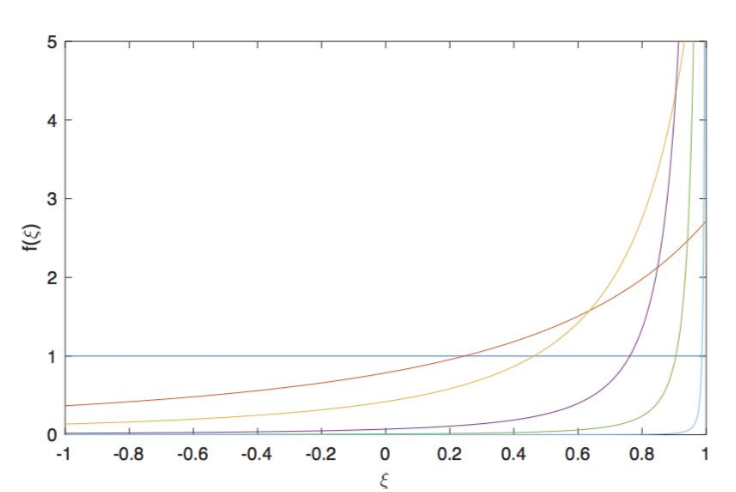
\includegraphics[width=.45\textwidth]{./Fig_notes/Fig1_note}
  \includegraphics[width=.45\textwidth,height=.4\textwidth]{./test3-Solution}\\
   \includegraphics[width=.9\textwidth,height=.6\textwidth]{./test3-TotalPartical} 
  %\footnotesize (a) & \footnotesize(b) 
\end{tabular}
\caption{Test \ref{Sect2-Ex3}: (a) Plot for solutions; (b) Total particles.}
\end{figure}

\paragraph{Example 4}\label{Test:Diffusion-Test4}
In this test, we shall assume the initial condition as
\begin{eqnarray*}
f_0(x)=\sum_{L=0}^\infty h_LP_L(x),
\end{eqnarray*}
where $P_L$ is the Legendre polynomial of degree $L$ and the coefficients are $h_0=3,\ h_1=0.5,\ h_2=1,\ h_3=0.7,\ h_4=3,\ h_6=3,$ and all other $h_L$ are set as zero.
\begin{figure}[H]
\centering
\begin{tabular}{cc}
 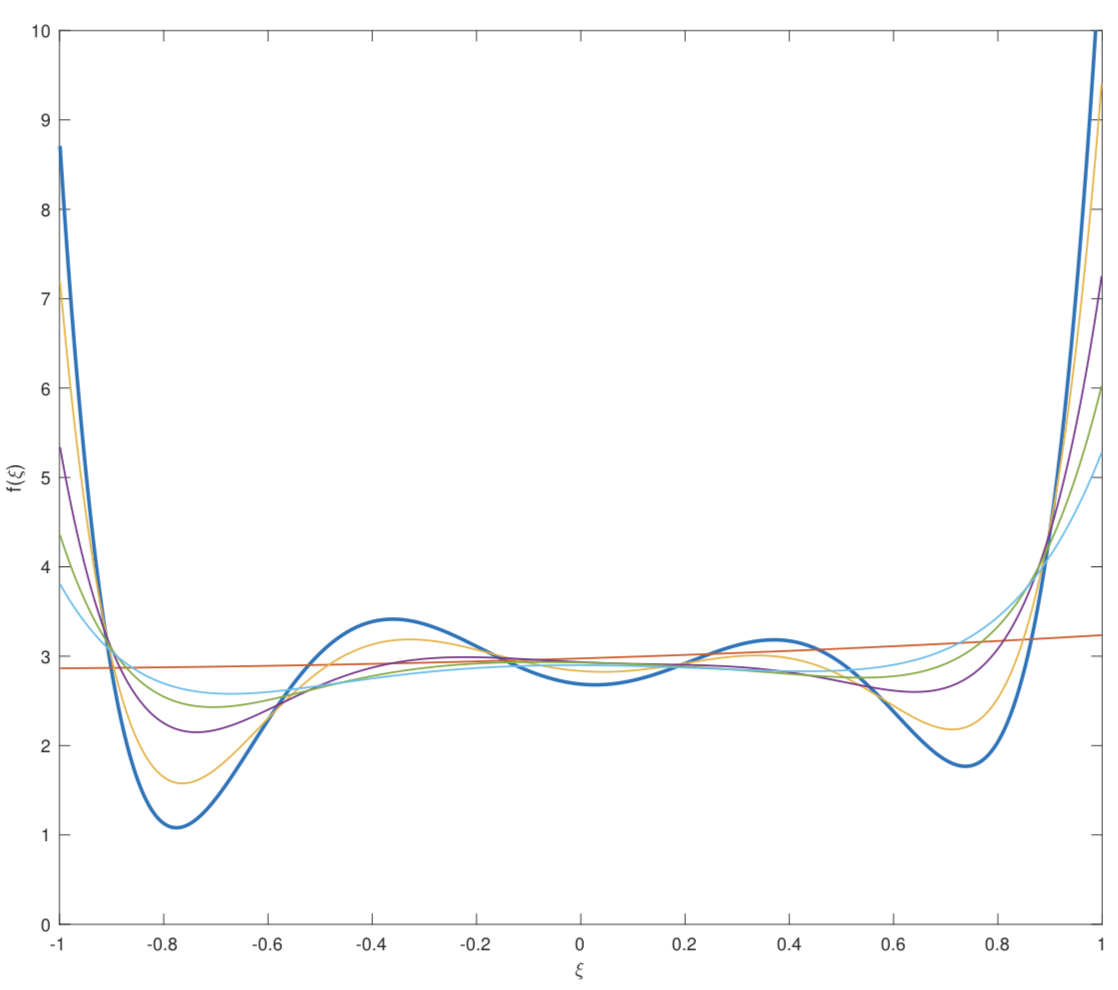
\includegraphics[width=.45\textwidth]{./Fig_notes/Fig3_note}
  \includegraphics[width=.45\textwidth,height=.4\textwidth]{./Diff-Deg5_Lev4}
  %\footnotesize (a) & \footnotesize(b) 
\end{tabular}
\caption{Test \ref{Test:Diffusion-Test4}: Numerical solution with Lev = 4 and Deg = 5; Notes (Left); Simulation (Right).}
\end{figure}

\subsection{Radiation Damping}
The evolution of the pitch angle dependence of $f$ in the presence of only radiation damping is governed by the equation
\begin{eqnarray}
\frac{\partial f}{\partial t} = -\frac{\partial}{\partial\xi}[\xi(1-\xi^2)f].
\end{eqnarray}

\subsubsection{Numerical Experiments}
The general solution is given by
\begin{eqnarray}
f(\xi,t)=\frac{\phi(1-\phi^2)}{\xi(1-\xi^2)}f_0(t),
\end{eqnarray}
where
\begin{eqnarray*}
\phi=\frac{\xi e^{-t}}{\sqrt{1-(e^{-2t}-1)\xi^2}}.
\end{eqnarray*}

alpha = 0

4 2 1.1562e-02   1.2294e-02
5 2 2.9780e-03   3.0811e-03
6 2 7.5420e-04   7.6794e-04

alpha = 1
4 2 6.4948e-02   7.7383e-02
5 2 3.2825e-02   3.9181e-02
6 2 1.6423e-02   1.9561e-02

alpha = 0
4 3 3.3562e-04   3.7930e-04
5 3 4.1533e-05   4.8142e-05
6 3 5.1423e-06   6.1385e-06



\subsection{Electric field and collisions}

Let
\begin{eqnarray*}
\frac{\partial f}{\partial t} =   C\frac{\partial}{\partial x}(1-x^2)\frac{\partial f}{\partial x}-E\frac{\partial}{\partial x}(1-x^2)f .
\end{eqnarray*}
First, we shall rewrite the equation as follows,
\begin{eqnarray*}
\frac{\partial f}{\partial t}+E\frac{\partial }{\partial x} (1-x^2)f &=& C\frac{\partial }{\partial x}q,\\
q - (1-x^2)\frac{\partial f}{\partial x}&=&0.
\end{eqnarray*}
Then the scheme becomes, to find $f_h,q_h\in V_h^k$, such that
\begin{eqnarray*}
&&\int_{I_j}\bigg(\frac{\partial f_h}{\partial t} - E (1-x^2) f_h \frac{\partial w}{\partial x}\bigg) dx +E\bigg( (\tilde{F}_{j+1/2})(w)^-_{j+1/2}-(\tilde{F}_{j-1/2})(w)^+_{j-1/2}\bigg)
\\
&&\quad\quad\quad\quad=-C\int_{I_j}q_h\frac{\partial w}{\partial x}dx + C\bigg( (\hat{Q}_{j+1/2})(w)^-_{j+1/2} -(\hat{Q}_{j-1/2})(w)^+_{j-1/2}\bigg),
\\
&&\int_{I_j}\bigg(q_h p-2xf_h p+(1-x^2)f_h\frac{\partial p}{\partial x}\bigg)dx-(\hat{F}_{j+1/2})(p)^-_{j+1/2}+(\hat{F}_{j-1/2})(p)^+_{j-1/2}=0,
\end{eqnarray*}
holds for $w,p\in V_h^k$, where $\tilde{F}_j$ is the upwind flux depending on the sign of $E$.
Here we shall assume $E\ge 0$ and take $\tilde{F}_{j+1/2}=(1-x_{j+1/2}^2)(f_h)_{j+1/2}^-$, $\tilde{F}_{j-1/2}=(1-x_{j-1/2}^2)(f_h)_{j-1/2}^-$, and alternating diffusion flux as follows,
\begin{eqnarray*}
\hat{Q}_{j+1/2}&=&(q_h)_{j+1/2}^+,\
 \hat{Q}_{j-1/2}=(q_h)_{j-1/2}^+
 \\
\hat{F}_{j+1/2}&=&{(1-x_{j+1/2}^2)}(f_h)_{j+1/2}^-,\
 \hat{F}_{j-1/2}={(1-x_{j-1/2}^2)}(f_h)_{j-1/2}^-.
\end{eqnarray*}

Thus, the matrix form reads
\begin{eqnarray*}
\begin{cases}
\dfrac{{\bf dF}_h}{dt} =& \mathbb{B}{\bf F}_h+\mathbb{A}_{2}{\bf Q}_h \\
{\bf Q}_h &= \mathbb{A}_{1} {\bf F}_h.
\end{cases}
\end{eqnarray*}
Thus, we can solve ${\bf F}^{n+1}$ explicitly by 3-rd Runge-Kutta methods for the following system:
\begin{eqnarray}
\frac{d{\bf F}_h}{dt} = R({\bf F}_h):= \mathbb{B}{\bf F}_h+\mathbb{A}_{2}\mathbb{A}_{1}{\bf F}_h.
\end{eqnarray}

%---------------------------
% Numerical Example
%---------------------------
\subsubsection{Numerical Test}
\paragraph{Example 1}\label{Sect1-Ex1}
In this test, we shall take domain as $\Omega=[-1,1]$, initial condition as $f_0(x)=1/2$  for testing.
\begin{figure}[H]
\centering
\begin{tabular}{c}
  \includegraphics[width=.95\textwidth]{./condiff-cf-E1}
  \end{tabular}
\caption{Test \ref{Sect1-Ex1}: Plot for solutions for Lev = 4, Deg = 5 of Central flux at time = 0.5, 1, 2, 2.5, 3.}
\end{figure}

\begin{figure}[H]
\centering
\begin{tabular}{c}
  \includegraphics[width=.95\textwidth]{./condiff-uf-E1_v2}
  \end{tabular}
\caption{Test \ref{Sect1-Ex1}: Plot for solutions for Lev = 4, Deg = 5 of upwind flux at time = 0.5, 1, 1.5, 2, 2.5, 3.}
\end{figure}

\begin{figure}[H]
\centering
\begin{tabular}{c}
  \includegraphics[width=.95\textwidth]{./condiff-uf-E2_v2}
  \end{tabular}
\caption{Test \ref{Sect1-Ex1}: Plot for solutions for Lev = 4, Deg = 5 of upwind flux at time = 0.5, 1, 1.5, 2, 2.5, 3.}
\end{figure}

\begin{figure}[H]
\centering
\begin{tabular}{c}
  \includegraphics[width=.95\textwidth]{./condiff-uf-E4_v2}
  \end{tabular}
\caption{Test \ref{Sect1-Ex1}: Plot for solutions for Lev = 4, Deg = 5 of upwind flux at time = 0.5, 1, 1.5, 2, 2.5, 3.}
\end{figure}

%\begin{figure}[H]
%\centering
%\begin{tabular}{c}
%  \includegraphics[width=.95\textwidth]{./condiff-uf-E1}
%  \end{tabular}
%\caption{Test \ref{Num-4}: Plot for solutions for Lev = 4, Deg = 5 of upwind flux at time = 0.5, 1, 1.5, 2, 2.5, 3.}
%\end{figure}
%
%\begin{figure}[H]
%\centering
%\begin{tabular}{c}
%  \includegraphics[width=.95\textwidth]{./condiff-uf-E2}
%  \end{tabular}
%\caption{Test \ref{Num-4}: Plot for solutions for Lev = 4, Deg = 5 of upwind flux at time = 0.5, 1, 1.5, 2, 2.5, 3.}
%\end{figure}
%
%\begin{figure}[H]
%\centering
%\begin{tabular}{c}
%  \includegraphics[width=.95\textwidth]{./condiff-uf-E4}
%  \end{tabular}
%\caption{Test \ref{Num-4}: Plot for solutions for Lev = 4, Deg = 5 of upwind flux at time = 0.5, 1, 1.5, 2, 2.5, 3.}
%\end{figure}



	


\subsection{Full Pitch Angle Dynamics}
The evolution of the pitch angle dependence of $f$ in the presence of electric field acceleration, collisions, and radiation damping is governed by the equation:
\begin{eqnarray}
\frac{\partial f}{\partial t}=-E\frac{\partial}{\partial\xi}[(1-\xi^2)f]+C\frac{\partial}{\partial\xi}[(1-\xi^2)\frac{\partial f}{\partial\xi}]-R\frac{\partial}{\partial\xi}[\xi(1-\xi^2)f],
\end{eqnarray}
where $E,C,$ and $R$ are constants. In this case, the steady state solution is given by
\begin{eqnarray}
f(\xi)=Q\exp[A\xi+(B/2)\xi^2],\ A=\frac{E}{C},\ B=\frac{R}{C},
\end{eqnarray}
with $Q$ as a normalization constant.

	\subsubsection{Numerical Scheme}
	Let $q=(1-\xi^2)\dfrac{\partial f}{\partial\xi}$, we re-write the above equation as follows,
	\begin{eqnarray*}
		\begin{cases}
	\dfrac{\partial f}{\partial t} &= -E\dfrac{\partial}{\partial\xi}[(1-\xi^2)f]+C\dfrac{\partial}{\partial\xi}q-R\dfrac{\partial}{\partial\xi}[\xi(1-\xi^2)f],\\
	q &= (1-\xi^2)\dfrac{\partial f}{\partial\xi}. 
		\end{cases}
	\end{eqnarray*}
	Then the corresponding variational forms are:
	\begin{eqnarray*}
	\int_{I_j}\frac{\partial f}{\partial t}v dx&=& E\int_{I_j}(1-\xi^2)f \frac{\partial v}{\partial \xi} dx - E\big(\tilde{F}_{j+1/2}v_{j+1/2}-\tilde{F}_{j-1/2}v_{j-1/2}\big)\\
	&& - C\int_{I_j} q \frac{\partial v}{\partial\xi} dx + C\big(\tilde{Q}_{j+1/2}v_{j+1/2}-\tilde{Q}_{j-1/2}v_{j-1/2}\big)\\
	&& + R\int_{I_j}\xi(1-\xi^2)f \frac{\partial v}{\partial \xi} dx - R\big(\tilde{P}_{j+1/2}v_{j+1/2}-\tilde{P}_{j-1/2}v_{j-1/2}\big)\\
	\int_{I_j} qw dx &=& -\int_{I_j}f\frac{\partial }{\partial\xi}[(1-\xi^2)w] dx + \big(\tilde{P}_{j+1/2}v_{j+1/2}-\tilde{P}_{j-1/2}v_{j-1/2}\big)
	\end{eqnarray*}

The boundary condition is assumed as follows:
\begin{eqnarray}
\frac{\partial f}{\partial\xi}|_{\xi = \pm 1,t} = 0.
\end{eqnarray}

\paragraph{Numerical Test}
The steady state solution is given by
\begin{eqnarray*}
f(\xi) = Q\exp\left[A\xi+(B/2)\xi^2\right],\ A = \frac{E}{C},\ B=\frac{R}{C}.
\end{eqnarray*}
Let $(A,B) = \{(0,4),(2,0),(2,2),(1,3)\}$ for testing.

\begin{figure}[H]
\centering
\begin{tabular}{c}
  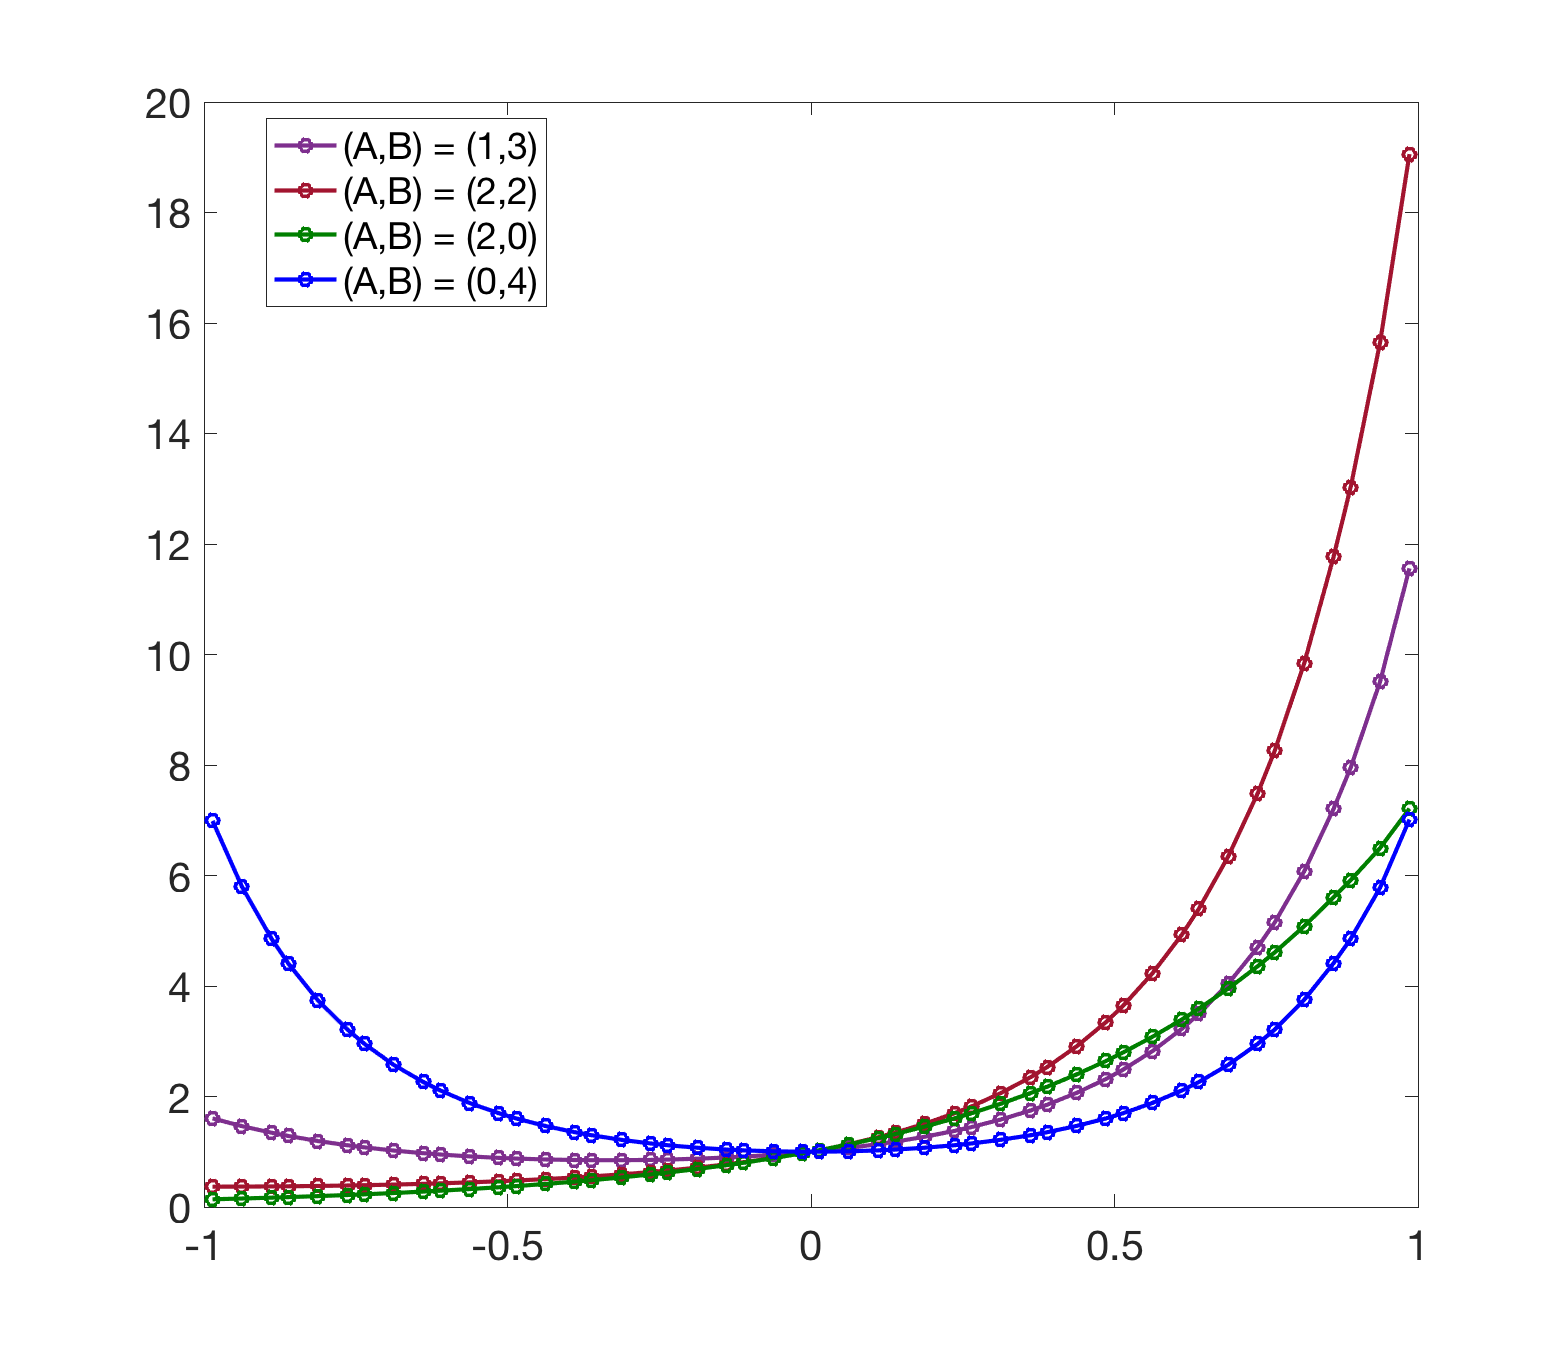
\includegraphics[width=.95\textwidth]{./test_full}
  \end{tabular}
\caption{Test }
\end{figure}


\section{Momentum Dynamics}
The full 1-D momentum dynamics is governed by the equation:
\begin{eqnarray}
\frac{\partial f}{\partial t}=\frac{1}{p^2}\frac{\partial}{\partial p}p^2\left[C_A\frac{\partial f}{\partial p}+C_Ff\right]-\frac{E}{p^2}\frac{\partial}{\partial p}\left[p^2f\right]+R\frac{1}{p^2}\frac{\partial}{\partial p}\left[p^3\gamma f\right]
\end{eqnarray}

\subsection{}
First, we shall consider the non-relativistic limit with $E=R=0$. That is, reduce the problem to the solution of 
\begin{eqnarray}
\frac{\partial f}{\partial t}&=&\frac{1}{x^2}\frac{\partial}{\partial x}x^2\left[\frac{\psi(x)}{x}\frac{\partial f}{\partial x}+2\psi(x)f\right]\notag\\
&=&\frac{1}{x^2}\frac{\partial}{\partial x}\left[ x\psi(x)\frac{\partial f}{\partial x}\right] + \frac{1}{x^2}\frac{\partial}{\partial x}\left[2x^2\psi(x)f \right].
\end{eqnarray}
Here $\psi(x) = \dfrac{1}{2x^2}\left[\dfrac{2}{\sqrt{\pi}}\int_0^{x}e^{-s^2}ds-\dfrac{2x}{\sqrt{\pi}}e^{-x^2}\right]=\dfrac{1}{2x^2}\left[\text{erf}(x)-\dfrac{2x}{\sqrt{\pi}}e^{-x^2}\right].$

\vskip.1in
Denote $q = \dfrac{\partial f}{\partial x}$ and rewrite the equation as follows:
\begin{eqnarray}
\begin{cases}
(q,v)_{I_i} &= \left(\dfrac{\partial f}{\partial x},v\right)_{I_i} ,\\
\left(x^2\dfrac{\partial f}{\partial t},w\right)_{I_i}  &= \left(\dfrac{\partial}{\partial x}\left[x\psi(x)q\right],w\right)_{I_i} +\left(\dfrac{\partial}{\partial x}\left[2x^2\psi(x)f\right],w\right)_{I_i} \\
& = -\left(x\psi(x)q,\dfrac{\partial w}{\partial x}\right)_{I_i} +\langle \widehat{x\psi(x)q},w\rangle_{\partial I_i} \\
&\quad -\left(2x^2\psi(x)f,\dfrac{\partial w}{\partial x}\right)_{I_i} +\langle \widehat{2x^2\psi(x)f},w\rangle_{\partial I_i} 
\end{cases}
\end{eqnarray}
Thus
\begin{eqnarray}
{\bf Q}^{n} &=& \textbf{Mat}_1*{\bf F}^{n}\\
\frac{{\bf F}^{n+1}-{\bf F}^n}{dt} &=& \textbf{Mat}_2*{\bf Q}^n + \textbf{Mat}*{\bf F}^n\notag\\
& = & \textbf{Mat}_2*\textbf{Mat}_1*{\bf F}^{n} + \textbf{Mat}*{\bf F}^n
\end{eqnarray}

Here $\textbf{Mat}_1$ is the Grad operator with FunCoef = 1. The matrix $\textbf{Mat}_2$ is the Grad operator with FunCoef = $x\psi(x)$, and the matrix $\textbf{Mat}$ is the Grad operator with FunCoef = $2x^2\psi(x)$.

\begin{figure}[H]
\centering
\begin{tabular}{c}
  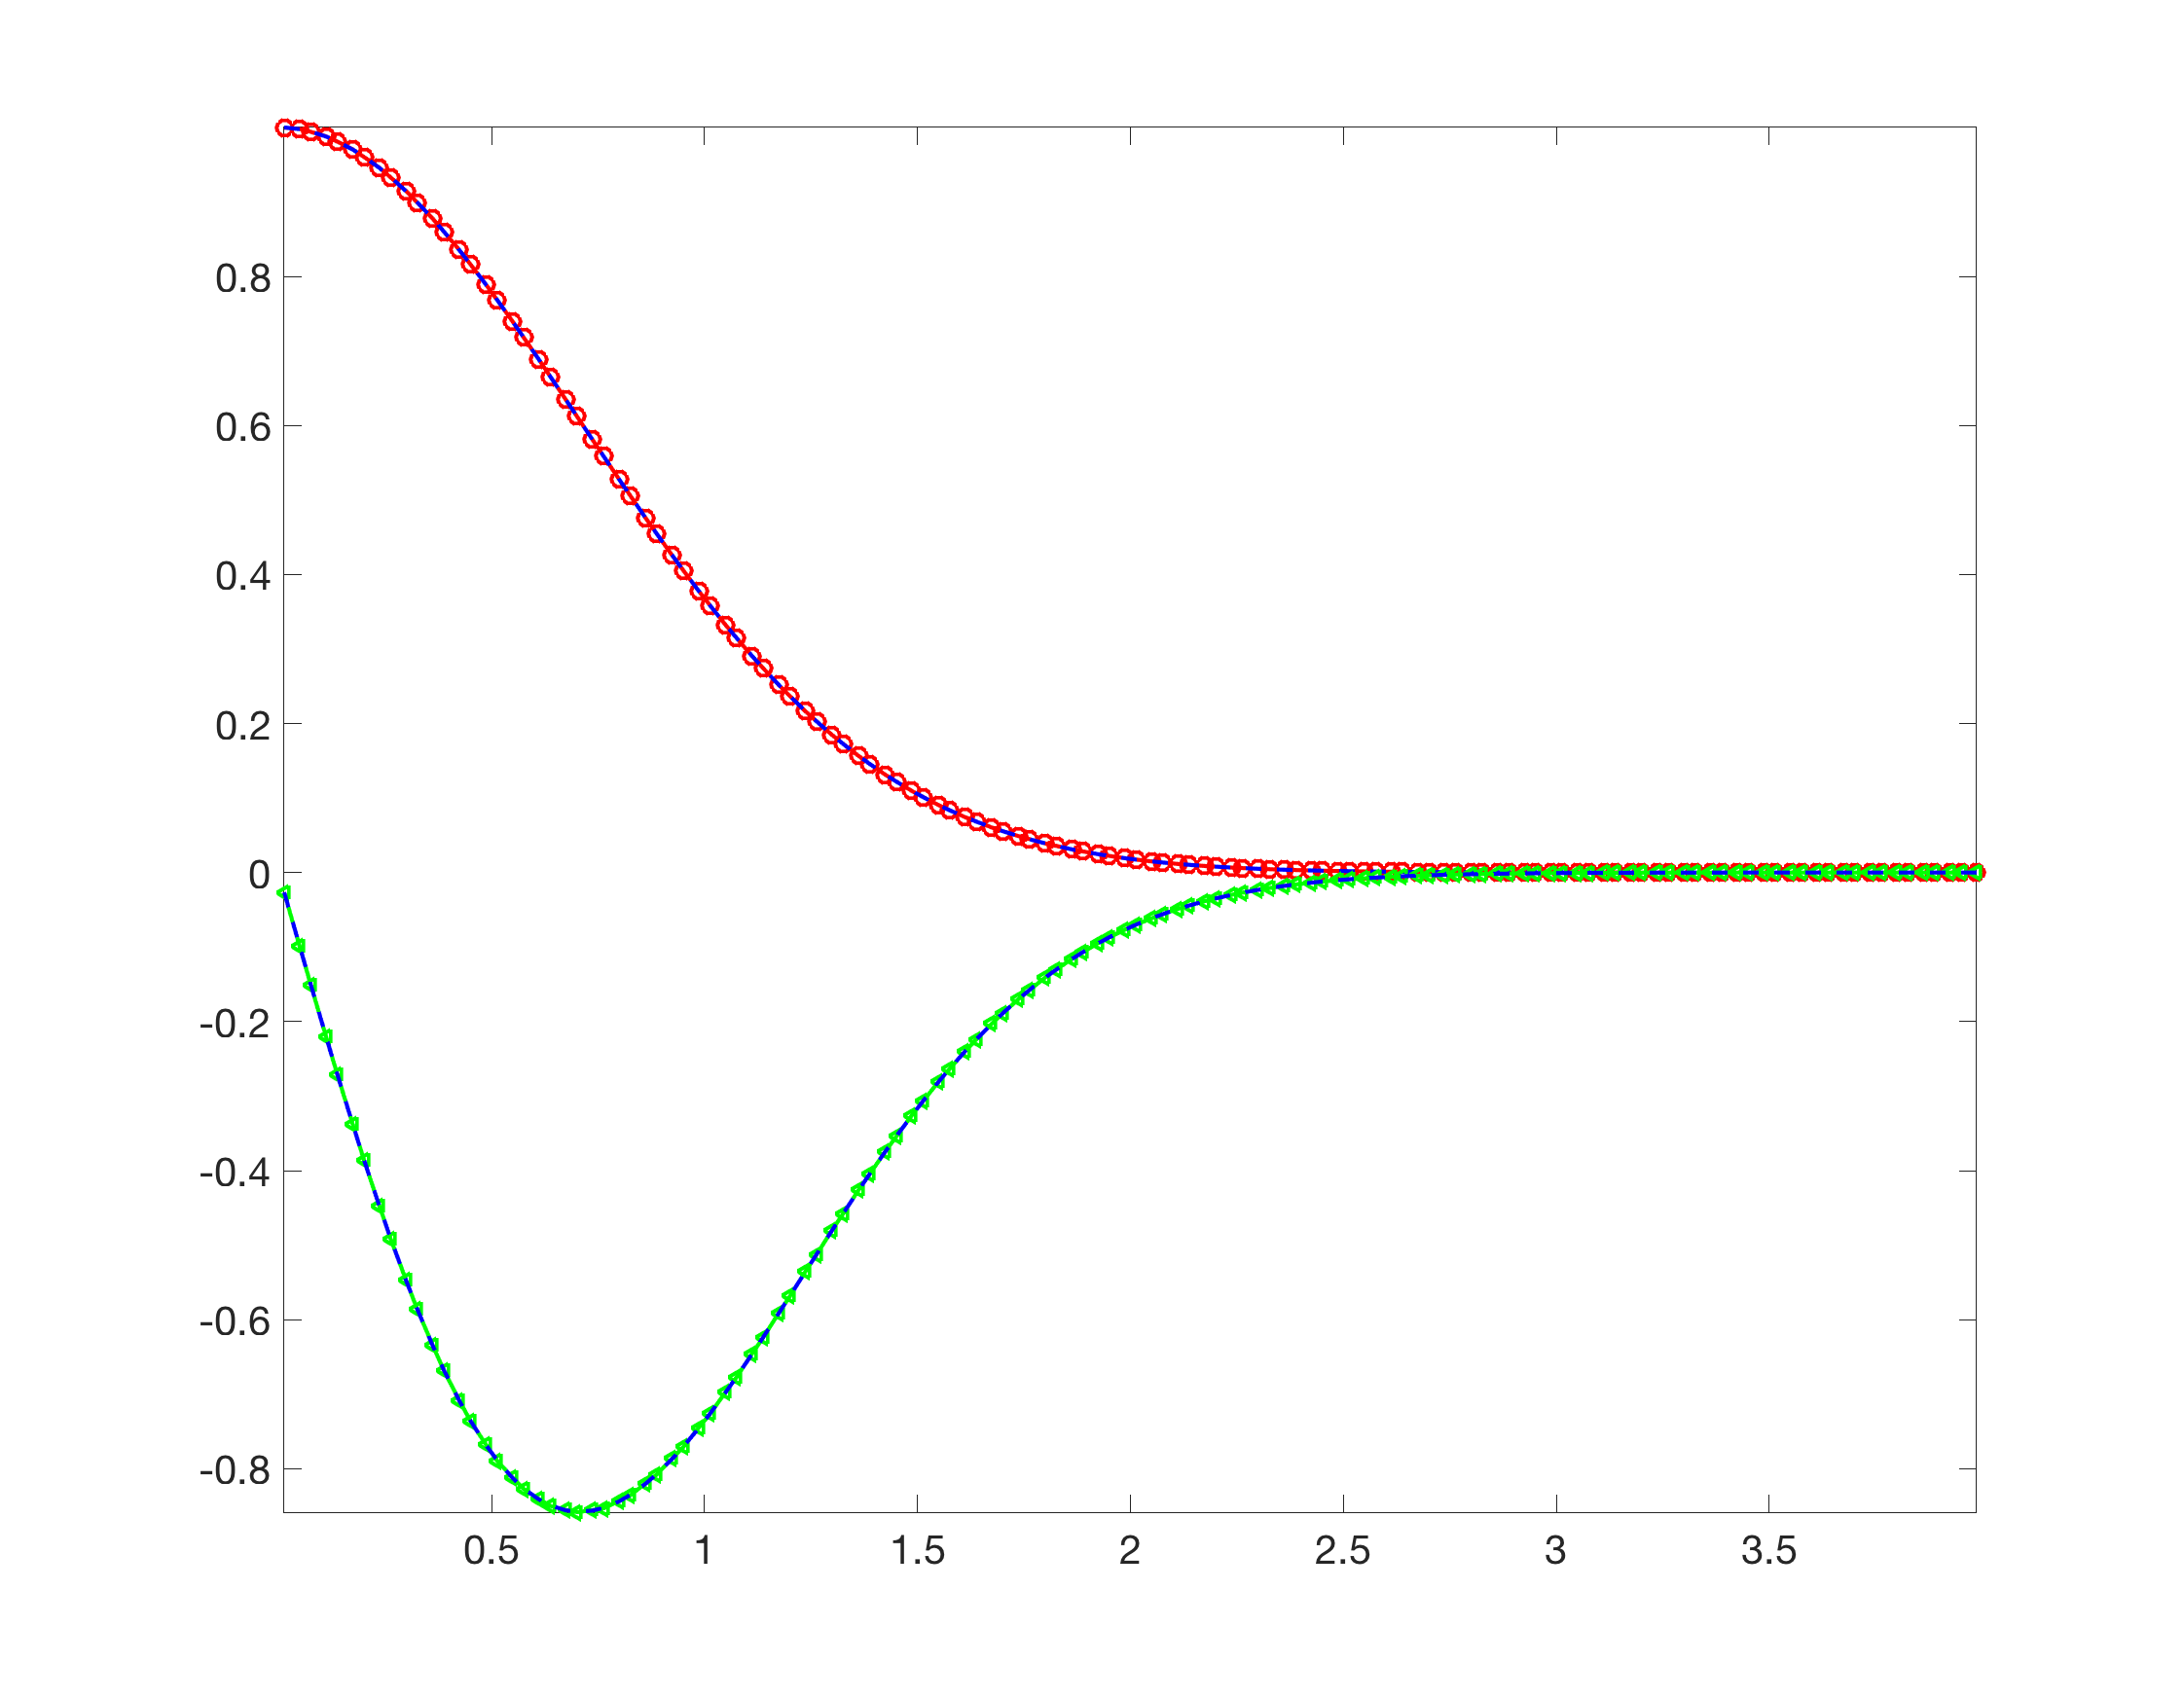
\includegraphics[width=.95\textwidth]{./test_mo.png}
  \end{tabular}
\caption{Test.}
\end{figure}


\begin{thebibliography}{99}

\bibitem{ShuOsher1988}
C.W. Shu and S. Osher. Efficient implementation of essentially non-oscillatory shock-capturing schemes. J. Comput.
Phys., 77 (1988):439-471.

\end{thebibliography}

\end{document}





